\documentclass[
%  master,
%  field=inf,
%  printversion,
%  biblatex,
%  language=czech,
%  font=sans,
  glossaries,
%  index
]{kidiplom}

\title{Domácí cloudové úložiště}
\title[english]{Home cloud storage}
\author{Aleš Kašpárek}
\supervisor{Mgr. Jan Tříska, PhD.}
\yearofsubmit{2021}
\annotation{Cílem práce je navrhnout a implementovat efektivní způsob uložení a sdílení souborů mezi uživateli, bez potřeby fyzického úložiště. Výsledkem práce je systém, pomocí kterého mohou uživatelé přistupovat ke svým souborům kdekoliv pomocí internetu.}
\annotation[english]{The main goal of thesis is to desing and implement effective way of storing and sharing files between users, without need of physical storage. Result of this thesis is a system, which allows users to use their files anywhere using the internet.}
\keywords{ cloud, cloudové úložiště, REST API, Python, GUI, C++, Docker}
\keywords[english]{cloud, cloud storage, REST API, Python, GUI, C++, Docker}
\thanks{Chtěl bych poděkovat Mgr. Janu Třískovi, PhD. za připomínky, nápady a zájem při tvoření této práce.}
\usepackage{lipsum}
\usepackage{float}

\begin{document}
\maketitle

\section{Úvod}
\label{sec:intro}
Cloud je v dnešní době velice oblíbené téma. Cloud lze popsat jako poskytování služeb nejčastěji dostupné přes prohlížeč nebo specializované aplikace, ke kterému lze přistupovat odkudkoliv přes internet. Cloud je provozována na virtualizovaném počítači, lokalizovaný na výkonných vzdálených serverech. Uživatel si poté pronajímá výkon těchto serverů. V dnešní době už u~mnoha firem nenajdeme rozsáhlá IT oddělení a přecpané serverovny, protože je pro ně mnohem pohodlnější pronajmout si výpočetní sílu cloudu. Mezi základní výhody patří:
\begin{itemize}
\item škálovatelnost,
\item aktuálnost software,
\item \uv{pay as you go} cenový model (platíme jen za to, co potřebujeme),
\item přístup přes internet \cite{WIKI_CLOUD}.
\end{itemize}
Distribuční model, který vypovídá o poskytovaných službách, obsahuje:
\begin{itemize}
\item IaaS - infrastruktura jako služba (servery a virtuální počítače (VM), úložiště, sítě a operační systémy),
\item Paas - platforma jako služba (na vyžádání doručují prostředí pro vývoj a testování a také poskytují a spravují softwarové aplikace),
\item SaaS - software jako služba (metoda doručování softwarových aplikací přes internet) \cite{MS_CLOUD}.
\end{itemize}

\subsection{Motivace}
Uložení dat a souborů v cloudu je jistě pohodlnější, než mít neustále po ruce fyzické úložiště. Jednak z hlediska sdílení mezi uživateli, tak z hlediska dostupnosti místa, kdy se uživatel nemusí obávat, zda-li ho má dostatek. 

Zvolené téma je v dnešní době velice diskutované, jelikož žádná z velkých organizací se o uložení vlastních dat nestará. Pro mnoho lidí je však problémem, že k jejich datům má poskytovatel služby přístup. Řešení, vypracované v této práci, nabízí uživatelům vlastní správu jejich dat.

Výsledná aplikace se poté skládá ze serveru, který se stará o samotné uložení a správu uživatelských dat, a desktopové aplikace, pomocí které uživatelé ke svým datům přistupují.

\clearpage
\section{Stávající cloudová řešení}
Většina stávajících řešení je zpoplatněná metodou předplatného. Za tuto cenu pak nabízejí různou velikost úložiště, kterou může uživatel využívat. Řada těchto služeb poskytuje i možnost bezplatného používání. Uživatelé jsou však v rámci této možnosti omezeni velikostí místa, které mohou využít. U bezplatného používání se velikost použitelného místa pohybuje v rámci jednotek gigabajtů, nejvíce pak 15\,GB. Platící uživatelé pak mohou využívat místo v řádech terabajtů. Následující sekce čerpá z \cite{CLOUDSOLUTIONS}.

\subsection{Google Drive}
Tato služba je přirozenou volbou pro vlastníky zařízení Android, ve kterých je služba integrována, ostatní uživatelé pak ocení 15\,GB prostoru.

S aplikací Google Photos pak mohou uživatelé se zařízením Android ukládat neomezené množství fotografií ve vysoké kvalitě. Po vylepšení na placený Google Drive uživatelé získají 2\,TB místa, se kterým mohou pracovat za cenu 99,99\,\$ ročně, a připojí se ke službě Google One.

Mezi výhody této služby patří integrovaná podpora u zařízení s operačním systémem Android, štědrá nabídka úložného prostoru pro neplatící uživatele a~neomezený počet zařízení spjatých s jedním účtem.

Nevýhodou služby je složité webové rozhraní. Uživatelé operačních systémů Windows a Mac si mohou stáhnout desktopovou aplikaci, která jim umožní nahrávat soubory přetažením.

\subsection{Microsoft OneDrive}
Podobně jako Google Drive zaměřený na uživatele Googlu, OneDrive je mířený na uživatele Microsoftu. Nabízí elegantní integraci s Outlook.com, populární e-mailovou platformou od této společnosti.

OneDrive se váže s Windows 10 a s celou řadou mobilních aplikací. Tím umožňuje přístup k souborům téměř odkudkoliv. Je také integrován se službami, které neposkytuje Microsoft, například s designovým gigantem AutoCAD.

Nabízí možnost sdílet soubory mezi uživateli, dokonce i s těmi, kteří sami nepoužívají OneDrive. Dále také možnost upravovat soubory online bez nutnosti stahování.

OneDrive pochází od gigantické společnosti Microsoft. Je tedy trochu zklamáním, že tato služba nabízí pro neplatící uživatele pouze 5\,GB místa, ale od 2\,\$ měsíčně mohou získat navýšení na 100\,GB.

Pokud uživatel vlastní Microsoft 365, dříve známý jako Office 365, získává k~němu automaticky 1\,TB úložiště s bezplatnou možností dalšího škálování. Musí mít však na paměti, že se jedná pouze o úložný prostor bez jakýchkoliv dalších pokročilých funkcí.

Za 79.99\,\$ ročně pak mohou uživatelé přejít na placený plán pro 6 uživatelů, který nabízí 6\,TB místa rozděleného mezi tyto uživatele. V rámci tohoto balíčku jsou zahrnuty další aplikace, například Word, Excel a další. \cite{ONEDRIVE}

\subsection{Dropbox}
Při porovnání s podobnými službami Dropbox podporuje relativně velký počet platforem od desktopu až po mobilní telefony. Nabízí celkem 10 klientů pro tyto platformy: Microsoft Windows, Mac OS a Linux (oficiální i neoficiální) a také pro oblast chytrých mobilních telefonů platforem Android, iPhone, iPad a~\mbox{BlackBerry}. Důležitým prvkem Dropboxu je také webové rozhraní služby pro ty, kteří nemají nainstalovaného klienta. Dropbox používá model financování Freemium, což znamená, že v základním provedení je zdarma a poskytuje nenáročným uživatelům 2\,GB úložiště s omezením datových přenosů na 20\,GB za den. U placených účtů je tento limit navýšen 2\,TB úložiště a 200\,GB přenosů za den. \cite{DROPBOX}

Zatímco Dropbox funguje i jako úložiště souborů, je zejména zaměřen na jejich synchronizaci a sdílení. Podporuje historii revizí, takže smazané soubory ze složky Dropbox mohou být kdykoliv obnoveny, a to jak přes webového klienta, tak i na kterémkoliv instalovaném klientu. Historie verzí je omezena na dobu 30\,dní, ale uživatelé mají možnost získat neomezenou historii zakoupením placené verze. Dojde-li ke změně souboru v synchronizované Dropbox složce, automaticky dojde k synchronizaci na všech připojených zařízeních. Výhodou Dropboxu je, že synchronizuje pouze tu část souboru, která se změnila, čímž omezuje využívání internetu na minimum. \cite{DROPBOX}

Základní platební plán pro jednotlivce vyjde na 9,99\,€ měsíčně, a obsahuje již zmíněné 2\,TB úložiště pro jednoho uživatele. Stejně jako bezplatný plán nabízí 30denní obnovu souborů a historii verzí. Rodinný plán za 16,99\,€ umožňuje přístup 6 uživatel, ale stále nabízí 2\,TB prostoru a obsahuje také stejnou 30denní obnovu souborů a historii verzí. \cite{DROPBOXPRICE}

\subsection{IDrive}
IDrive nabízí synchronizaci souborů, dokonce i souborů na síťových discích. Webové rozhraní umožňuje sdílení přes e-mail, Facebook a Twitter. Opatrní uživatelé rádi uslyší, že smazání souboru z počítače neznamená smazání souboru ze serveru, což znamená menší nebezpečí náhodného smazání něčeho důležitého.

Je zachováno až 30 předešlých verzí souborů na uživatelově účtu. Další věc, kterou je třeba poznamenat, je, že správci mají přístup k aplikaci IDrive Thin Client, která jim umožňuje zálohovat a obnovovat, spravovat nastavení atd. pro všechna jejich připojená zařízení prostřednictvím centralizovaného řídicího panelu.

Pro fotografie nabízí funkci rozpoznání obličeje, které pomáhá při organizaci fotografií. IDrive také nabízí službu IDrive Express, která uživateli v případě ztráty dat nabízí zaslání fyzického pevného disku, umožňující rychlé obnovení zálohovaných souborů.

IDrive nabízí hned několik možností předplatného. Základní bezplatný plán nabízí 5\,GB využitelného místa. Další nabídka je 5, popř. 10\,TB, které stojí 52,12\,\$, popř. 74,62\,\$ a nabízí přístup pro jednoho uživatele z neomezeného množství počítačů. Další plán začíná s přístupem z 5 počítačů, 5\,TB místa a přístupu 5 uživatelů a škáluje až na 50 počítačů a uživatelů a 50\,TB prostoru. Poslední nabídka také obsahu hned několik nabídek různých velikostí úložiště, k tomu nabízí neomezený počet uživatelů, počítačů a serverů, mimo jiné také službu Exchange, SQL a také synchronizaci souborů na síťových discích a začíná na 74,62\,\$. \cite{IDRIVEPRICE}

\subsection{Backblaze}
Backblaze je gigant v odvětví cloudových úložišť, průmyslový veterán, který se stará jak o osobní, tak o velké obchodní zálohy. Klíčové slovo je zde \uv{záloha}, jelikož nenabízí žádnou synchronizaci ani kolaboraci. Backblaze nabízí zálohu, to je vše. Jako jediný nabízí skutečné neomezené cloudové úložiště, bez jakýchkoliv dalších závazků.

Cena předplatného pro osobní zálohy, která může být placena měsíčně, ročně, nebo v období 2 let, je velice výhodná (60\,\$ za rok), zvláště bereme-li v úvahu neomezenou velikost úložiště.

Mezi výhody Backblaze tedy patří neomezená velikost úložiště, jednoduchost a společně při nákupu s ExpressVPN pak nízká cena. Na rozdíl od předchozích zmíněných řešení nenabízí kromě zálohování žádnou jinou funkci a uživatelům umožňuje přístup pouze z jednoho počítače.

\subsection{pCloud}
Tato služba jako jedna z mála nabízí možnost doživotního předplatného a uživatel v podstatě získá permanentní virtuální cloudovou jednotku. Služba se popisuje jako \uv{osobní cloudový prostor, kde můžete ukládat všechny svoje soubory a~složky s uživatelsky přívětivým rozhraním, které jasně ukazuje, kde se všechno nachází, a co dělá.}


pCloud nabízí 30denní historii koše a neomezenou rychlost nahrávání, uživatelé jsou však omezeni velikostí stahování 500\,GB pro Premium a 2\,TB pro Premium Plus za měsíc.

Od srpna 2020 také umožňuje uživatelům vybrat, zda-li chtějí mít svoje data uložená na serverech v Evropě nebo v Americe. Společnost samotná je registrovaná ve Švýcarsku, které má přísné zákony pro soukromí, a proto nabízí možnost zaplatit 4,99\,\$ měsíčně za pCloud Crypto k zamčení (a odemčení) jednotlivých souborů heslem.

pCloud nabízí dvě možnosti předplatného. Patří sem služba Premium, která nabízí 500\,GB prostoru, sdílení mezi uživateli a 30denní koš za cenu 47,88\,€ ročně, nebo 175\,€ jednorázově na doživotí. Druhou možností je Premium Plus, nabízející 2\,TB a také sdílení a 30denní koš. Za tuto možnost uživatelé zaplatí 95,88\,€ ročně, nebo 350\,€ jednorázově. \cite{PCLOUD}

\subsection{Srovnání stávajících řešení a výsledné aplikace}
Výsledná aplikace nabízí uložení souborů a jejich sdílení mezi uživateli. Hlavním rozdílem oproti komerčním řešením jsou její nízké náklady a fakt, že si uživatelé spravují svá data sami. Právě fakt, že k datům nemají přístup třetí strany, je hlavním rozdílem od stávajících řešení.
Téměř všechna současná řešení vyžadují po uživateli předplatné. Mezi další výhodu tohoto řešení patří jeho nízká cena. Uživatel zaplatí pouze za hardware, na kterém bude spuštěný server, a za úložiště. Dále si sám může vybrat velikost úložiště, které bude používat.

K 3.5.2021 se cena tohoto řešení pohybuje do 4000\,Kč. Tato cena se může měnit v závislosti na vybraném Raspberry Pi. Je možné vybírat z několika variant, každá varianta se liší velikostí paměti RAM a procesorem. Dále je v této ceně zahrnuto samotné fyzické úložiště. Je možné vybrat jednoduchý flash disk s kapacitou v řádu gigabajtů, za to však s nižší cenou, nebo popřípadě hard disk s vyšší kapacitou, o to však vyšší cenou.

\clearpage
\section{Použité technologie}
Aplikace je založena na komunikaci klienta se serverem. Proto bylo velice důležité vybrat nástroj, který umožní snadný a rychlý vývoj serveru a jeho následné nasazení. Dále pak bylo potřeba vybrat nástroj pro sestrojení klientské aplikace, která poběží na operačních systémech Windows a Linux. Posledním úkolem bylo zajištění hardwaru pro server. Bylo vybráno Raspberry Pi 4, které nabízí přijatelný výkon za nízkou cenu a nízkou spotřebu energie.

\subsection{Server}
Hlavními kritérii pro výběr technologie pro server byla snadná manipulace s~HTTP požadavky, jednoduché sestrojení REST API, které funguje na výše zmíněném HTTP protokolu, a jednoduchá práce s JSON soubory.

Vedlejšími faktory při výběru byla jednoduchá práce s databází, podpora frameworku Swagger pro jednoduchý vývoj REST API a nezávislost na operačním systému. Nakonec byl zvolen programovací jazyk Python a balíček Connexion pro sestrojení API.

Následně pak byl server nasazen za pomoci nástroje Docker, který umožňuje běh serveru bez závislosti na operačním systému a architektuře procesoru.

\subsubsection{Docker}
Docker je open-source platforma pro vývoj, nasazení a spouštění aplikací. Umožňuje zabalit a spustit aplikaci 	ve volně izolovaném prostředí nazývaném kontejner. Izolace a zabezpečení umožňují běh několika kontejnerů najednou. Kontejnery jsou nenáročné a obsahují vše potřebné pro běh aplikace a na rozdíl od virtuálních strojů, které vyžadují hypervisor, jsou spuštěny přímo v rámci kernelu operačního systému. \cite{DOCKER}

\begin{figure}[htp]
    \centering
    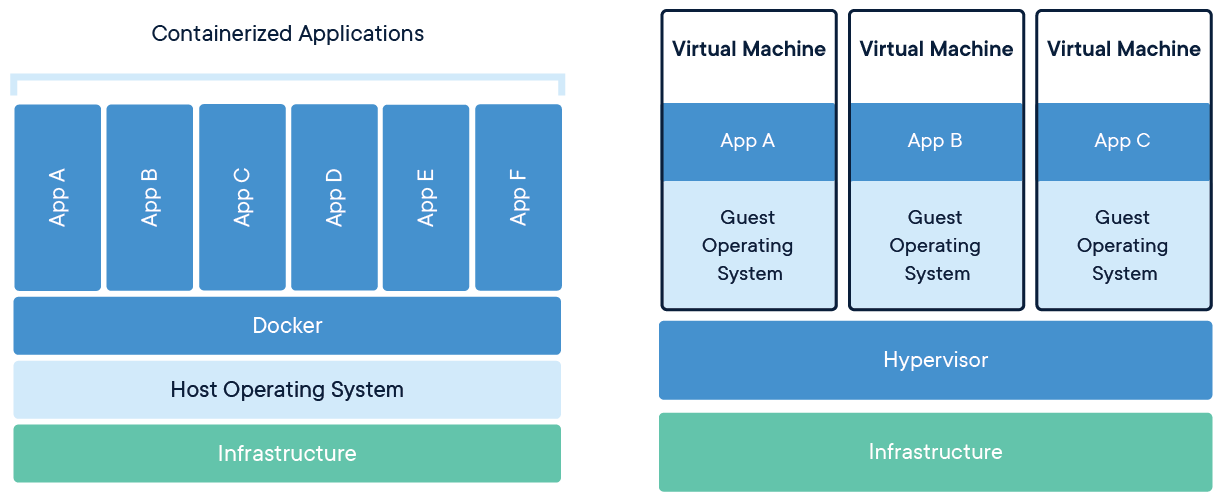
\includegraphics[width=10cm]{Docker-containerized-and-vm-transparent-bg}
    \caption{Srovnání dockeru a virtuálních strojů \cite{DOCKERIMAGE}}
    \label{fig:DockerSchema}
\end{figure}

\clearpage

\subsubsection{Python/Connexion}
Python je interpretovaný, objektově orientovaný, vysokoúrovňový programovací jazyk s dynamickou kontrolou datových typů. Podporuje moduly a balíčky, které zvyšují modularitu programu a znovupoužitelnost kódu. \cite{PYTHON}

Connexion je framework postavený na Flasku, který automaticky zpracovává HTTP požadavky definované použitím OpenAPI (dříve známé jako Swagger). Connexion umožňuje psát specifikaci (ukázka kódu~\ref{code:EndpointExample}) a poté mapuje endpointy (kontaktní body, pomocí kterých dochází k interakci API s ostatními systémy), definované v~této specifikaci, na pythonové funkce. Toto je rozdíl od ostatních nástrojů, které generují specifikace podle kódu. \cite{CONNEXION}

\begin{kicode}{tex}{code:EndpointExample}{Ukázka specifikace}
paths:
  /apistatus:
    get:
      tags: 
        - API management
      summary: Health status of application
      description: Checks database availability and API response threshold time.
      operationId: manager.api_status.ApiStatus.get
      responses:
        200:
          description: API is healthy
        400:
          description: API is down
\end{kicode}

\subsection{Klientské části}
Dalším a neméně důležitým cílem bylo vytvoření aplikace, která bude spustitelná na počítačích s operačními systémy Windows a Linux. Pro klientskou aplikaci byl vybrán framework Qt, který umožňuje vývoj aplikací s uživatelským rozhraním v jazyce C++. Tento framework také umožňuje psát jeden kód, který funguje na obou operačních systémech.

Jelikož však C++ v základu neposkytuje tvorbu HTTP požadavků, práci se soubory ve formátu JSON, ani deterministickou hashovací funkci, bylo potřeba vybrat knihovny, které tuto funkčnost poskytnou.

\subsubsection{C++}
C++ je univerzální multiparadigmatický programovací jazyk vytvořený jako rozšíření programovacího jazyka C. Jazyk postupem času narostl, a moderní C++ je nyní objektově orientované, generické, má funkcionální rysy spolu s nízkoúrovňovou správou paměti. Téměř vždy je implementován jako kompilovaný jazyk. \cite{C++}


Bylo však nutné do standartní knihovny přidat další funkcionalitu zajišťující:
\begin{itemize}
\item Vytváření HTTP požadavků - knihovna libcurl, vývojová knihovna nástroje curl \cite{LIBCURL}.
\item Manipulaci s JSON soubory - knihovna nlohmann/json, přidává podporu pro manipulaci s JSON objekty podobnou jazyku Python \cite{JSONCPP}.
\item Deterministickou hashovací funkci - knihovna openssl, implementuje protokoly SSL a TLS \cite{OPENSSL}.
\end{itemize}
S pomocí těchto nástrojů bylo možné se pustit do samotného vývoje.

\subsubsection{Qt}
Qt je multiplatformní framework široce používaný pro vytváření aplikací s grafickým uživatelským rozhraním určeným pro rozličné softwarové a hardwarové platformy. Qt je knihovna programovacího jazyka C++, ale existuje i pro jazyky Python (PyQt, PySide), Ruby (QtRuby), C, Perl, Pascal, C\#, Java (Jambi) a Haskell. Velkou výhodou Qt je velmi přehledně zpracovaná dokumentace a také vývojové programy Qt Creator nebo Qt Designer. Aplikace vytvořené pro grafické uživatelské prostředí používají nativní vzhled operačního systému, takže vyvinuté aplikace se vždy přizpůsobí vzhledu používaného prostředí \cite{QT}.

\clearpage
\section{Server}
Tato část se věnuje struktuře serveru a její implementaci. 
\subsection{Integrace databáze}
Jako databáze byl vybrán dockerový image Postgres, který byl vybrán jakožto open-source databázový systém. Dále bylo nutné napojit samotný server k této databázi. K tomuto byl použit pythonový balíček Peewee. Zároveň bylo nutné vyřešit čekání serveru na inicializaci databáze.

\subsubsection{Čekání na databázi}
Čekání na databázi zajišťuje vstupní bod, ve kterém běží smyčka dotazování se na databázi. Toto čekání bylo nutné implementovat, protože by mohlo dojít k~situaci, kdy se uživatel bude snažit o připojení k serveru krátce po jeho spuštění, ale databáze ještě nebude inicializována. V tomto případě bude na server zaslán požadavek o autentizaci, ale server nebude mít přístup k databázi a nebude moci ověřit přihlašovací údaje, a tento požadavek skončí chybou.
\begin{kicode}{bash}{code:WaitForDB}{Mechanismus čekání na databázi}
until python3 utils/wait_for_db.py -eq 0 ; do
    echo "Waiting for database to initialize"
    sleep 2;
done
\end{kicode}

\subsubsection{Peewee}
Peewee je pythonový balíček, který nabízí objektově relační mapování. Jinými slovy mapuje data z relační databáze na objekty vytvořené programovacím jazykem. Peewee podporuje všechny operace, které nabízí relační databáze bez nutnosti psát výrazy v jazyce SQL.

\subsubsection{Databázové třídy}
Databázové třídy odrážejí strukturu datového modelu. Bylo nutné vybrat vhodné datové typy, vyřešit relace mezi tabulkami, dále také povinné a nepovinné parametry.
\begin{itemize}
\item Jméno tabulky určuje atribut \texttt{table\_name} metatřídy, od které je třída odvozena.
\item Identifikátorem záznamu byl zvolen typ UUID, který slouží k jedinečné identifikaci záznamu a je automaticky generován při každém zápisu. Kód~\ref{code:model} na řádku 7.
\item Atributy, které mohou nabývat hodnoty \texttt{NULL}, mají argument \texttt{null} nastaven na hodnotu \texttt{True} a naopak. Kód~\ref{code:model} na řádku 8.
\item Cizí klíče jsou reprezentovány hodnotou \texttt{ForeignKeyField}. Tento cizí klíč je dále specifikován třídou, která odpovídá příslušné tabulce, a názvem sloupce. Kód~\ref{code:model} na řádku 16 a 17.
\end{itemize}

\begin{kicode}{python}{code:model}{Třídy databázové tabulky}
class BaseModel(Model):

    class Meta:
        database = DB

class NtwUsers(BaseModel):
    id = UUIDField(primary_key=True)
    user_name = TextField(null=False, unique=True)
    passw = TextField(null=False, unique=False)

    class Meta:
        table_name = "ntw_users"
        schema = SCHEMA_NAME
        
class Share(BaseModel):
    from_user = ForeignKeyField(NtwUsers, to_field='id')
    to_user = ForeignKeyField(NtwUsers, to_field='id')
    directory = TextField(null=False)
    file_name = TextField()

    class Meta:
        table_name = "share"
        schema = SCHEMA_NAME
        primary_key = False
\end{kicode}

\subsubsection{Metatřída a základní model}
Všechny třídy reprezentující databázové tabulky dědí ze základní třídy. V této třídě je specifikováno, ke které databázi se vztahují. Zde je specifikován atribut \texttt{database}, který obsahuje samotné připojení k databázi, má nastavené přihlašovací jméno a heslo, a mimo jiné i slovník. Tento slovník slouží k mapování datových typů jazyka SQL na datové typy definované programátorem. Bylo nutné jej použít, jelikož Peewee v základu nenabízí typ UUID.

V metatřídách jednotlivých databázových tříd je poté nastaveno několik dalších informací. Například je zde definován název tabulky a schéma, ve kterém se tabulka nachází, nebo je zde také uveden záznam, že daná tabulka neobsahuje žádný primární klíč.

\clearpage

\subsection{Struktura API}
\begin{figure}[htp]
    \centering
    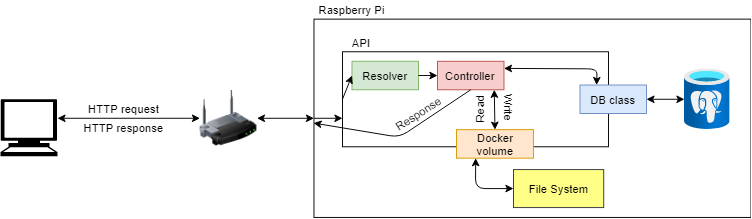
\includegraphics[width=15cm]{API_diagram}
    \caption{Schéma struktury API}
    \label{fig:APISchema}
\end{figure}

\subsubsection{Směrování}
Server ve výchozím nastavení naslouchá na portu 8000. Pro přístup zařízení, které se nachází ve stejné síti, byl tento port zachován, ale pro zařízení, které se připojuje z jiné sítě, bylo nastaveno směrování portů z portu 80 na port 8000.

\subsubsection{API endpointy}
Endpointy definují samotnou strukturu API. Sestávají se z metod, které obsluhují jednotlivé HTTP požadavky.
\begin{kicode}{python}{code:endpoint}{Ukázka kódu endpointu}
class FilePostHandler(PostRequest):

    @classmethod
    def handle_post(cls, **kwargs):
        filePath = DISK_PATH + kwargs["user"] + kwargs["directory"]
        file = kwargs["fileName"]
        incomingFileSize = os.fstat(file.fileno()).st_size
        _, _, free = shutil.disk_usage(DISK_PATH)
        if incomingFileSize > free:
            return cls.format_exc("Internal server error", 500,"Not enough free space.") 
        savePath = filePath + str(unicodedata.normalize('NFKD', file.filename).encode('ascii', 'ignore'))[2:-1]
        file.save(savePath)
        return 200
\end{kicode}
\clearpage
Tento endpoint je definován pomocí OpenAPI následovně:

\begin{kicode}{python}{code:endpointDefinition}{Definice endpointu}
  /files/{user}:
    post:
      tags: 
        - File handling
      summary: Post a file.
      description: Post a file.
      operationId: manager.files.FilePostHandler.post
      ...
\end{kicode}


Atribut \texttt{operationId} na řádku 7 v ukázce~\ref{code:endpointDefinition} definuje jaká metoda bude daný endpoint obsluhovat. Endpoint pro kód~\ref{code:endpointDefinition} obsluhuje požadavky na adrese  \mbox{\textit{[adresa\_serveru]/files/\{user\}}}.

Protokol HTTP dovoluje použítí 8 metod \cite{HTTPmethods}, ale v práci byly použity pouze 3 z nich. U jejich používání byla dodržována jejich definice:
\begin{itemize}
	\item GET- Metoda sloužící pouze k získávání dat ze serveru.
	\item POST - Metoda pro zasílání dat na server.
	\item DELETE - Metoda pro smazání všech výskytů zdroje z URI. 
\end{itemize}

Tento endpoint reaguje pouze na POST requesty, jak je možné vidět na řádku~2 v kódu~\ref{code:endpointDefinition}.

\subsubsection{Docker volume}
Volumes jsou preferovaným mechanismem pro persistentní data generovaná a~používaná kontejnery. \cite{DOCKERvolume}

Docker volume je jednoduchý nástroj, kterým bylo docíleno jednoduchého zapisování a odesílání souborů. Je velice snadné volume vytvořit za pomoci souboru docker-compose.yaml.
\begin{kicode}{python}{code:dockerVolume}{Definice docker volume}
        volumes:
            - /media/pi/KINGSTON/NAS:/tmp/NAS
\end{kicode}

Část před dvojtečkou odkazuje do souborového systému v rámci hostitelského systému. Část po dvojtečce udává, kde se v rámci kontejneru tyto soubory nachází. Jinými slovy to, co je v kontejneru uloženo v \textit{/tmp/NAS}, bude fyzicky uloženo v \textit{/media/pi/KINGSTON/NAS}.

\subsubsection{OpenAPI a dokumentace}
Nástroj OpenAPI (dříve známý jako Swagger) automaticky zpracovává strukturu API z YAML nebo JSON souboru a následně ji poskytuje v podobě webové stránky a JSON souboru. Tento nástroj byl zvolen jakožto nejjednodušší způsob udržování dokumentace. Vizuální dokumentaci API endpointu je možné vidět na obrázku~\ref{fig:openapi}.

\begin{figure}[htp]
    \centering
    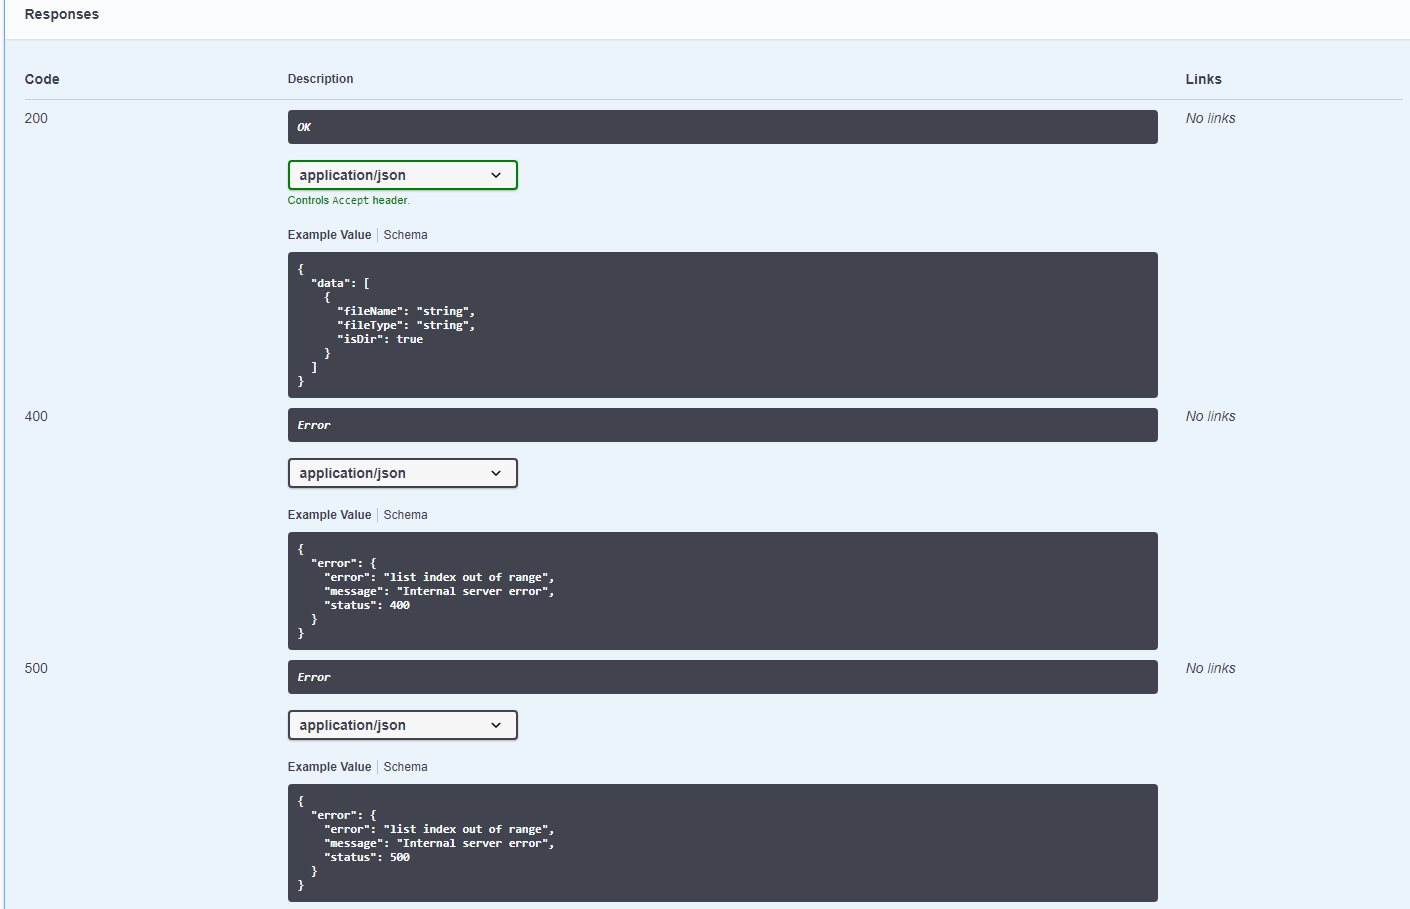
\includegraphics[width=14cm,height=10cm,keepaspectratio]{openapi}
    \caption{Ukázka grafické dokumentace OpenAPI}
    \label{fig:openapi}
\end{figure}

Tato stránka sloužila k otestovaní a debuggování jednotlivých endpointů. Je možné ji nalézt na adrese \mbox{\textit{[adresa\_serveru]/ui/}}. Nabízí jednoduchou vizualizaci odpovědí, které jsou získané od jednotlivých endpointů. Dále nabízí vytváření a zasílání požadavků na server s vlastními argumenty, které jsou poté předány funkcím obsluhující jednotlivé endpointy API.

\clearpage
\subsubsection{Vývoj a debuggovací mód}
Jelikož server běží na Raspberry Pi, bylo žádoucí celý vývoj přesunout právě na něj, což však nebylo příliš komfortní. Právě proto nabízí Visual Studio Code rozšíření, které umožňuje využít protokolu SSH, aby bylo možné pokračovat ve vývoji odkudkoliv.

Během vývoje bylo mnohokrát nutné některé endpointy složitě debuggovat. K~ladění byl použit balíček ptvsd, který implementuje debugger pro použití v programu Visual Studio Code. Dále bylo nutné v rámci kontejneru povolit port 5678, na kterém tento debugger funguje, a nastavit proměnnou prostředí \texttt{DEBUG}. Tato proměnná udává, má-li se má server spustit v debuggovacím módu. Následně bylo nutné povolit debuggování v kódu, jak je ukázáno v ukázce~\ref{code:debugMode}. Posledním požadavkem pro ladění bylo nakonfigurování debuggeru programu Visual Studio Code pro Python: Remote Attach. 
\begin{kicode}{python}{code:debugMode}{Zahájení debuggeru}
    if debug_mode:
        import ptvsd
        LOGGER.info("WAITING FOR DEBBUGER")
        ptvsd.enable_attach(address = ('0.0.0.0', 5678), redirect_output=True)
        ptvsd.wait_for_attach()
\end{kicode}
\clearpage
\section{Klientské části}
Tato část se věnuje implementaci uživatelské aplikace a také obsahuje uživatelskou dokumentaci.

\subsection{Dostupné platformy}
Aplikace byla vyvinuta a její zamýšlené nasazení se vztahuje na operační systémy Windows a Linux.

\subsubsection{Komunikace aplikace se serverem}
Veškerou komunikaci obstarává knihovna libcurl \cite{LIBCURL}, která zasílá požadavky na server a přijímá odpovědi. Tyto odpovědi mohou být následujícího typu:
\begin{itemize}
	\item požadovaný soubor - v tom případě je uložen do složky vytvořené v dočasných souborech následně v závislosti na operačním systému:
	\begin{itemize}
	\item Windows - je zavolána funkce \textit {ShellExecuteA} poskytovaná rozhraním Windows API, které požadovaný soubor otevře pomocí výchozí aplikace pro jeho otevření.
	\item Linux - je zavolána funkce \textit{fork}, která vytvoří nový proces a v tomto procesu je provedeno volání \textit{execl} s argumentem \textit{"/usr/bin/xdg-open"}. Tento soubor je poté otevřen v novém procesu opět pomocí výchozí aplikace.
	\end{itemize}
	\item JSON soubor - v tomto případě se knihovna \mbox{nlohmann/json} \cite{JSONCPP} postará o parsování odpovědi, která je následně zpracována.
\end{itemize}
\subsection{Uživatelská dokumentace}
\subsubsection{Dialog pro zadání IP adresy}
Při úplně prvním spuštění aplikace se uživateli zobrazí dialog pro zadání IP adresy zařízení, na kterém běží server a port. Uživatel je dotázán na veřejnou IP adresu a na adresu, kterou zařízení má v domácí síti. Je velmi důležité, aby na routeru bylo nastavené směrování portů na port serveru a do příslušného zařízení. Uživatel je po potvrzení přesměrován na přihlašovací dialog. Pro účel této práce jsem přidal zaškrtávací políčko \textit{Use default}, které automaticky doplní adresu serveru běžícího na Raspberry Pi.
\begin{figure}[H]
    \centering
    \includegraphics[width=8cm,height=7cm,keepaspectratio]{ip}
    \caption{Dialog pro zadání IP adres}
    \label{fig:ip}
\end{figure}
\subsubsection{Přihlašovací dialog}
Při každém dalším spuštění je uživateli ukázán přihlašovací dialog. Zde si uživatel může buď vytvořit nový účet, nebo se přihlásit ke stávajícímu. Po potvrzení dialogu je zaslán požadavek na server o autorizaci uživatele. Během autorizace ještě na straně klienta dochází k použití algoritmu SHA-256 \cite{SHA256} z~knihovny OpenSSL \cite{OPENSSL} k vytvoření hashe z hesla, jelikož hesla jsou v databázi uložena v hashované podobě, aby nikdo nemohl vidět, jaké heslo si uživatel zvolil. Ještě před odesláním hesla je k němu přidána tzv. \uv{sůl}, která dělá těžším dešifrování hesla. Poté je buď ukázána chybová hláška, že uživatel zadal špatné přihlašovací údaje, nebo dochází k zobrazení dialogu pro samotnou manipulaci se soubory.

V tomto dialogu si také uživatel po zvolení možnosti \texttt{Sign~In} v menu může založit účet, pomocí kterého bude poté manipulovat se soubory.
\subsubsection{Uživatelské soubory}
\begin{figure}[H]
    \centering
    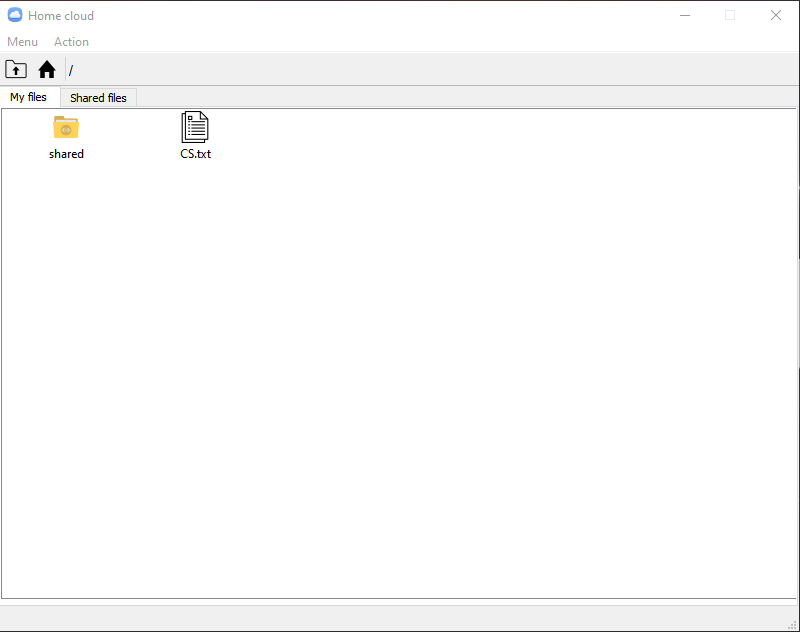
\includegraphics[width=14cm,height=10cm,keepaspectratio]{MainWindow}
    \caption{Uživatelova hlavní obrazovka}
    \label{fig:usersworkspace}
\end{figure}
V hlavním okně má uživatel možnost procházet svoje soubory a soubory sdílené od ostatních uživatelů. Může také vytvořit složku kliknutím pravého tlačítka myši a vybráním možnosti \textit{Create folder}, nebo také nahrát nové soubory možností \textit{Upload file}. To samé může udělat buď z hlavní nabídky možností \textit{Action} a~následně \textit{Upload}, nebo prostým přetáhnutím souboru, který chce nahrát. Dále, pokud má uživatel vybraný soubor a klikne na něj pravým tlačítkem myši, má možnost jej smazat možností \textit{Delete}, nebo jej sdílet s ostatními uživateli vybráním \textit{Share with...}.

Toto okno mimo jiné obsahuje pole, které indikuje ve které složce se uživatel nachází. Obsahuje také ovládací prvky, kterými se uživatel pohybuje ve stromové struktuře. První ovládací prvek slouží k přesunutí o složku výš, a druhý k~okamžitému přesunutí do kořenové složky.

\subsubsection{Sdílené soubory}
\begin{figure}[H]
    \centering
    \includegraphics[width=14cm,height=10cm,keepaspectratio]{shared}
    \caption{Záložka se sdílenými soubory}
    \label{fig:shared}
\end{figure}
Uživatel může kdykoliv přepnout na záložku se soubory sdílenými od ostatních uživatelů. Jako první si uživatel vybere od koho chce sdílené soubory zobrazit a~poté už vidí přímo sdílené soubory. Sdílet se mohou samostatné soubory i~složky. Při sdílení složek dochází ke sdílení veškerého obsahu uvnitř složky. Když uživatel soubor smaže, dochází také automaticky k ukončení sdílení.

I v tomto případě má uživatel k dispozici ovládací prvky sloužící k navigaci ve stromové struktuře.

\subsection{Nasazení aplikace}
Aplikace je distribuována instalátorem. Pro tvorbu tohoto instalátoru jsem využil knihovnu Qt Installer Framework \cite{QTINSTALLER}. Tento framework umožňuje snadno a~rychle vytvářet instalační soubory pro projekty Qt a podporuje operační systémy Microsoft Windows, Linux a macOS.
\clearpage
\section{Příručka vlastního spuštění server}
Jediným požadavkem pro spuštění serveru je mít nainstalovanou službu Docker. Proto byl do projektu přidán skript \textit{install.sh}, který tuto službu nainstaluje. Dále je nutný docker-compose, který tento skript také nainstaluje. K instalaci docker-compose je použit program pip. Je zamýšleno, že server poběží pouze na operačním systému Linux, a program pip je už předinstalovaný.

Druhý skript, \textit{start.sh}, poté slouží ke spuštění serveru.

\subsection{Statická IP adresa}
Uživatel by před samotným během serveru měl zajistit, aby stroji na kterém běží byla přidělena statická IP adresa v rámci sítě. Tento krok je nezbytný jak v~rámci přístupu v domácí síti, tak v rámci přístupu z jiného místa. Jelikož je nutné nastavit směrování portů, bez statické IP adresy by nemusely HTTP požadavky na server dorazit.

\subsection{Nastavení úložiště}
Nastavení úložiště se provádí nastavím docker volume, jak je možné vidět na řádku 2 v kódu~\ref{code:dockerVolume} v souboru \textit{docker-compose.yaml}. Uživatel pouze nastaví část před dvojtečkou na cestu, kam by chtěl, aby se mu soubory ukládaly.
\clearpage
\section{Možnosti dalšího vývoje}
Tento projekt zatím nabízí pouze uložení souborů a do budoucna existuje celá řada vylepšení a přidání dalších funkcí. 

Vytváření náhledových obrázků pro uložené soubory je první věcí, která by byla do projektu přidána. Tato změna bude představovat zjednodušení uživatelského rozhraní, jelikož se uživatelé ve svých souborech pomocí těchto náhledů budou lépe orientovat.

Dalším funkcí je streamování souborů ze serveru. Ať už jde o obrázky nebo videa, streamování je zajisté jednodušší než soubor stáhnout a poté ho otevřít. V rámci této změny by měla také být přidána možnost editovat soubory.

Do budoucna by také měla být představena mobilní aplikace, jak pro telefony s operačním systémem Android, tak pro iOS. Uživatelé tak budou mít své soubory po ruce, i když zrovna nejsou u počítače.

V poslední řadě by celý projekt měl být otevřený veřejnosti jako open-source, jelikož otevřený software nabízí neomezené množství nápadů a náhledů na toto řešení.

\begin{kiconclusions}
Výsledek splnil svůj hlavní cíl, tedy vytvoření domácího cloudového úložiště. Aplikace umožňuje snadný přístup k souborům uloženým na vzdáleném serveru, umožňuje správu uživatelů a sdílení souborů mezi uživateli. Vytvořená aplikace je schopná fungovat na operačních systémech Windows a Linux. Způsob vývoje dovoluje aplikaci doplnění o další funkcionalitu a zvolený způsob nasazení umožňuje snadné použití.

Výsledné řešení nabízí cenově dostupné cloudové úložiště, kde si sami uživatelé spravují svá data. Vyznačuje se snadným sestavením a instalací a téměř neomezenou modulárností. Zvolený způsob nasazení umožňuje serveru běžet na jakémkoliv hardwaru. Zároveň je také možné k následnému uložení použít jakýkoliv typ úložiště.

Systém však také nabízí celou řadu vylepšení do budoucna, ať už se jedná o přidání další funkcionality, nebo například o design moderního uživatelského rozhraní, které odpovídá moderním desktopovým aplikacím.

Projekt také bude představovat přínos pro open-source komunitu, ve které se bude dále vyvíjet.

\end{kiconclusions}

\begin{kiconclusions}[english]
The result met the main goal, which was to create a home cloud storage. The application allows easy access to files stored on a remote server, user management and sharing files between users. Created application is able to run on Windows and Linux operating systems. Method of development allows to add additional funcionality to system and chosen method of deployment allows easy use of applicatoion.

The resulting solution offers affordable cloud storage, where users manage their own data. It is characterized by easy assembly and installation and almost unlimited modularity. The chosen deployment method allows the server to run on any hardware. At the same time, it is also possible to use any type of storage for subsequent storage.

However, the system also offers a number of improvements in the future, whether it is the addition of additional functionality or, for example, the design of a modern user interface that corresponds to modern desktop applications.

The project will also be of addition to the open-source community, in which it will continue to develop.

\end{kiconclusions}

\begin{thebibliography}{Cloud}
	\bibitem[1]{WIKI_CLOUD} Cloud computing - Wikipedie. [online]. Dostupné z: 
		\url{https://cs.wikipedia.org/wiki/Cloud\_computing}
	\bibitem[2] {MS_CLOUD} Co je cloud computing? Průvodce pro začátečníky | Microsoft Azure [online]. Dostupné z: 
		\url{https://azure.microsoft.com/cs-cz/overview/what-is-cloud-computing/\#cloud-computing-models}
	\bibitem[3]{DOCKER} Docker overview | Docker Documentation. [online]. Dostupné z:
		\url{https://docs.docker.com/get-started/overview/}
	\bibitem[4]{PYTHON} What is Python? Executive Summary | Python.org [online].
	Dostupné z:
		\url{https://www.python.org/doc/essays/blurb/}
	\bibitem[5]{CONNEXION} Welcome to Connexion’s documentation! — Connexion 2.0 documentation [online]. Dostupné z: 
		\url{https://connexion.readthedocs.io/en/latest/}
	\bibitem[6]{C++} C++ - Wikipedia [online]. Dostupné z:
		\url{https://en.wikipedia.org/wiki/C++}
	\bibitem[7]{QT} Qt (knihovna) – Wikipedie [online]. Dostupné z:
		\url{https://cs.wikipedia.org/wiki/Qt\_(knihovna)}
	\bibitem[8]{DOCKERvolume} Use volumes | Docker Documentation [online]. Dostupné z:
		\url{https://docs.docker.com/storage/volumes/}
	\bibitem[9]{HTTPmethods}  HTTP request methods - HTTP | MDN [online]. Dostupné z:
		\url{https://developer.mozilla.org/en-US/docs/Web/HTTP/Methods}
	\bibitem[10]{LIBCURL}  libcurl - the multiprotocol file transfer library [online]. Dostupné z:
		\url{https://curl.se/libcurl/}
	\bibitem[11]{JSONCPP}  nlohmann/json: JSON for Modern C++ [online]. Dostupné z:
		\url{https://github.com/nlohmann/json}
	\bibitem[12]{OPENSSL}  OpenSSL [online]. Dostupné z:
		\url{https://www.openssl.org/}
	\bibitem[13]{SHA256}  Secure Hash Algorithm – Wikipedie [online]. Dostupné z:
		\url{https://cs.wikipedia.org/wiki/Secure\_Hash\_Algorithm}
	\bibitem[14]{QTINSTALLER} Qt Installer Framework Manual [online]. Dostupné z:
		\url{https://doc.qt.io/qtinstallerframework/index.html}
	\bibitem[15]{DOCKERIMAGE} File:Docker-containerized-and-vm-transparent-bg.png - Wikimedia Commons [online]. Dostupné z:
		\url{https://commons.wikimedia.org/wiki/File:Docker-containerized-and-vm-transparent-bg.png}
	\bibitem[16]{CLOUDSOLUTIONS} Best cloud storage services for 2021 | TechRadar [online]. Dostupné z:
		\url{https://www.techradar.com/news/the-best-cloud-storage}
	\bibitem[17]{DROPBOX} Dropbox – Wikipedie [online]. Dostupné z:
		\url{https://cs.wikipedia.org/wiki/Dropbox}
	\bibitem[18]{ONEDRIVE} Cloud Storage Pricing and Plans – Microsoft OneDrive [online]. Dostupné z:
		\url{https://www.microsoft.com/en-ww/microsoft-365/onedrive/compare-onedrive-plans?market=af}
	\bibitem[19]{DROPBOXPRICE} Compare All Dropbox Plans ‐ Dropbox [online]. Dostupné z:
		\url{https://www.dropbox.com/plans?tab=personal}
	\bibitem[20]{IDRIVEPRICE} IDrive® pricing plans [online]. Dostupné z:
		\url{https://www.idrive.com/pricing}
	\bibitem[21]{PCLOUD} pCloud - Best Cloud Storage Pricing \& Cost Plans [online]. Dostupné z:
		\url{https://www.pcloud.com/cloud-storage-pricing-plans.html}
\end{thebibliography}
\clearpage

\appendix
\section{Obsah přiloženého CD/DVD} \label{sec:ObsahCD}
\begin{description}

\item[\texttt{desktop\_app/}] \hfill \\
 Složka s aplikací. Obsahuje instalační soubory pro Windows a Linux. Dále obsahuje zdrojový kód desktopové aplikace.

\item[\texttt{server/}] \hfill \\
   Složka obsahující zdrojové kódy serveru.
   
\item[\texttt{theses/}] \hfill \\
Složka se textem práce a jeho zdrojovým kódem.

\item[\texttt{readme.txt}] \hfill \\
  Instrukce pro spuštění.
 

\end{description}

\end{document}
